La figura de este ejercicio muestra un objeto $AB$ colocado frente a una lente convergente, y las posiciones de los focos de ésta.
\begin{enumerate}
    \item Trace el diagrama que permita localizar la imagen de este objeto proporcionada por la lente.
    \item La imagen obtenida, ¿es real o virtual? ¿Es derecha o invertida? ¿Y mayor o menor que el objeto?
\end{enumerate}
\begin{figure}[h!]
  \centering
  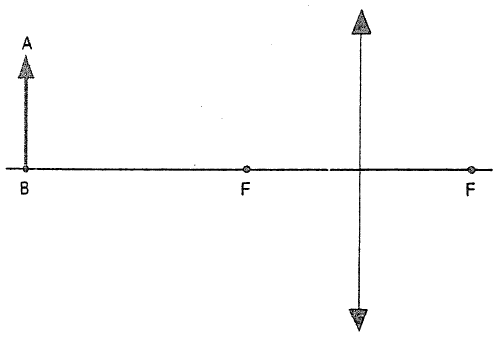
\includegraphics[scale=0.45]{figuras/fig_alvarenga_p687_25.png}
  \caption{Problema 15}
\end{figure}